\section{Uncertainty of Sniffer Trace}
\label{sec:model}

Two underlying properties of the communication medium are assumed in this paper:
non-zero packet loss probability and physical diversity.
%
Suppose the DUT communicates with an endpoint using certain protocol, the
non-zero packet loss means the sniffer could miss packets from the DUT or the
endpoint.
%
Physical diversity property means each device's packet reception probability is
independent with each other.
%
Therefore, it is possible for a packet to be received by the sniffer but missed
by the DUT, or vice versa.
%
Note that we use the term \textit{sniffer} to refer to a logical entity that can
observe the DUT's behavior. It may consist of multiple physical devices and the
traces from different devices are fused to provide one unified
view~\cite{Cheng:2006:JSP:1159913.1159920,Mahajan:2006:AMB:1159913.1159923}.

For wireless networks, the above two assumptions are natural.
%
However, we note that the assumptions are also applicable to wired networks over
multiple hops.
%
Consider a sniffer deployed on one of the intermediate hops, a packet could be
dropped before or after reaching the destination, causing different observation
between the sniffer and either of the end points.
%
Or the packets could be temporally routed via alternate paths, bypassing the
sniffer. 

To summarize, a sniffer could either miss packets seen by the DUT, or capture
extra packets that are missed by the DUT. It is precisely such incompleteness of
sniffer packet traces that brings uncertainty to the validation problem.

\begin{figure}[t!]
  \centering
  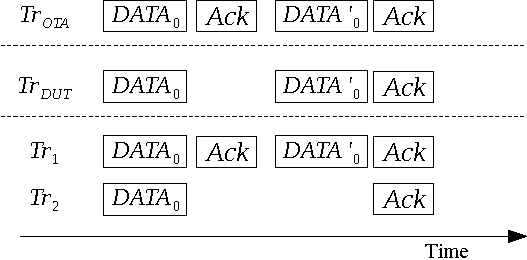
\includegraphics[width=0.45\textwidth]{./figures/false_pos.pdf}
  \caption{\textbf{Uncertainty Caused by Sniffer Observations.} $Tr_{OTA}$ is
    the chronological sequence of packets sent by the DUT and the endpoint.
    $Tr_{DUT}$ is the trace of the DUT. $Tr_1$ and $Tr_2$ are two possible traces
  of the sniffer.}
  \label{fig:sniffer_in_middle}
\end{figure}

Consider the 802.11 data transmission protocol and a few example traces observed by
sniffers shown in Figure~\ref{fig:sniffer_in_middle}.
%
The transmitter (DUT) sends a packet $DATA_0$.
%
Even though the receiver (endpoint) receives $DATA_0$ and sends out an $Ack$
packet, the DUT does not receive the $Ack$ packet.
%
Eventually the acknowledgment timer fires and the DUT retransmits $DATA_0$
(denoted as $DATA'_0$) and receives the acknowledgment.
%
It is obvious that the DUT obeys the protocol with respect to its own
observation $Tr_{DUT}$.

In first possible sniffer trace $Tr_1$ where the sniffer \textit{overhears} the
first $Ack$ packet, a validation \textit{uncertainty} arises when the sniffer
sees the retransmission packet $DATA'_0$: was the previous $Ack$ missed by the
DUT or is there a bug in DUT which causes it to retransmit even after receiving
the $Ack$?
%
Similarly, consider another possible sniffer trace
$Tr_2$ where both the $DATA'_0$ and $Ack$ packets were missed by the sniffer.
%
During this period of time, it appears the DUT neither receives acknowledgment
for $DATA_0$ nor retransmits $DATA'_0$.
%
Again, without any additional information it is impossible to disambiguate between the
sniffer missing certain packets and a bug in DUT's retransmission logic.

Assume that the endpoint implementation is correct, \textbf{given the expected
behavior of the DUT and the sniffer's observation with inherent uncertainty, can
we validate that the DUT behaves as specified by the protocol?}
%
This is the question we set out to answer in this paper.
